\cotefile{69}
\scanpage{85}

\diagram{%
\begin{tikzcd}[ampersand replacement=\&,row sep=small,column sep=small]
 A_3\ {\text{ép.}} \\
 A_4\ {\text{ép.}}\arrow[u,"4"] \&[-1.5em]
 {\sim A_5\ {\text{ép.}}\sim\text{hex. ép.}\sim\text{prisme épinglé}\sim\text{carrés ép.}}\\
 \text{\unsure{carroussel|carrousel} ép.}\sim\text{pent. épi}\arrow[u,"3"]\\
 (\text{\unsure{repères|repère}})\arrow[u,"2"]
\end{tikzcd}%
}

\diagram{%
\begin{tikzcd}[ampersand replacement=\&,column sep=0pt,row sep=0pt]
|[inner sep=0pt]| \vcenter{\hbox{%
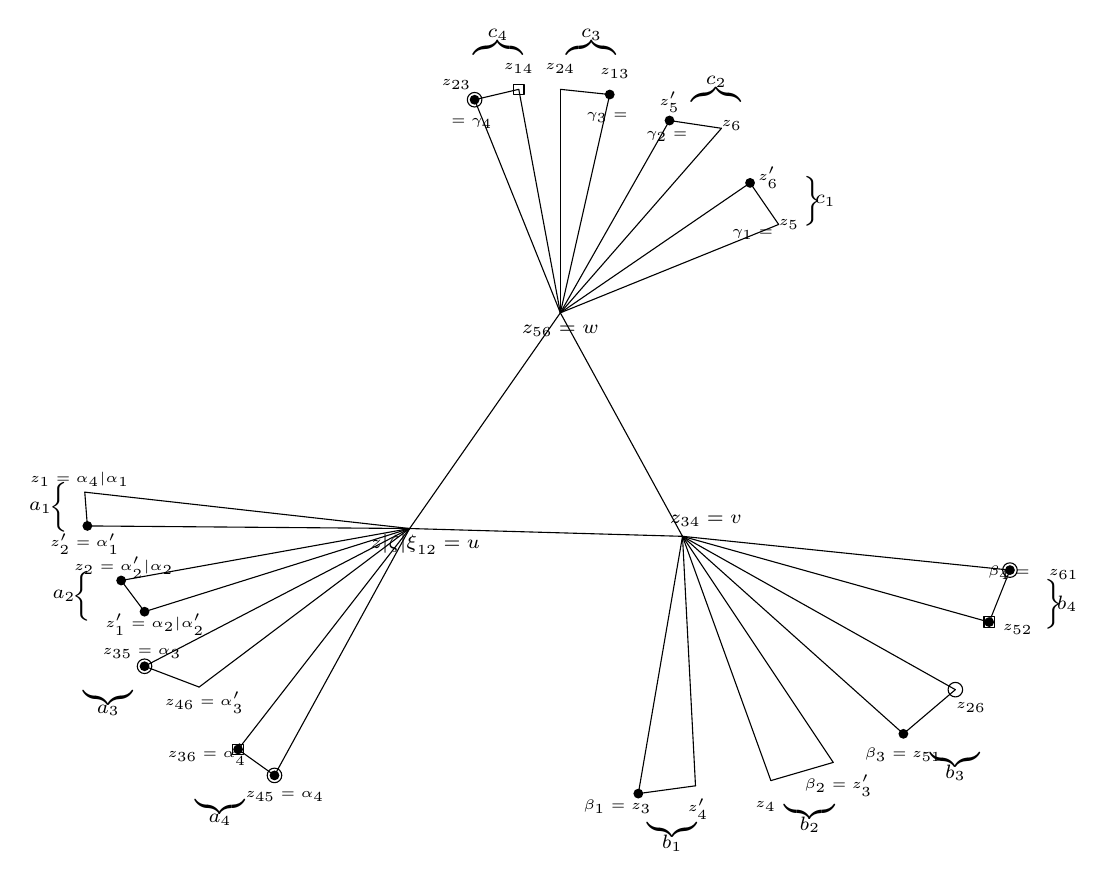
\begin{tikzpicture}[x=0.033cm,y=-0.033cm,line cap=round,line join=round,line width=.4pt]
\draw (142,165) -- (247,168) -- (200,82) -- cycle;
\node[inner sep=.55pt,anchor=center,font=\scriptsize] at (148,171) {$\unsure{z|\zeta|\xi}_{12}=u$};
\node[inner sep=.55pt,anchor=center,font=\scriptsize] at (256,162) {$z_{34}=v$};
\node[inner sep=.55pt,anchor=center,font=\scriptsize] at (200,89) {$z_{56}=w$};
\draw (142,165) -- (17,151);
\draw (142,165) -- (18,164);
\draw (17,151) -- (18,164);
\draw (142,165) -- (31,185);
\draw (142,165) -- (40,197);
\draw (31,185) -- (40,197);
\draw (142,165) -- (40,218);
\draw (142,165) -- (61,226);
\draw (40,218) -- (61,226);
\draw (142,165) -- (76,250);
\draw (142,165) -- (90,260);
\draw (76,250) -- (90,260);
\fill (18,164) circle[radius=0.0625cm];
\fill (31,185) circle[radius=0.0625cm];
\fill (40,197) circle[radius=0.0625cm];
\fill (40,218) circle[radius=0.0625cm];
\fill (76,250) circle[radius=0.0625cm];
\fill (90,260) circle[radius=0.0625cm];
\draw (74,248) -- (78,248) -- (78,252) -- (74,252) -- cycle;
\draw (40,218) circle[radius=0.0925cm];
\draw (90,260) circle[radius=0.0925cm];
\node[inner sep=.55pt,anchor=center,font=\tiny] at (15,146) {$z_1=\unsure{\alpha_4|\alpha_1}$};
\node[inner sep=.55pt,anchor=center,font=\tiny] at (17,171) {$z'_2=\alpha'_1$};
\node[inner sep=.55pt,anchor=center,font=\tiny] at (32,180) {$z_2=\unsure{\alpha'_2|\alpha_2}$};
\node[inner sep=.55pt,anchor=center,font=\tiny] at (44,202) {$z'_1=\unsure{\alpha_2|\alpha'_2}$};
\node[inner sep=.55pt,anchor=center,font=\tiny] at (39,213) {$z_{35}=\unsure{\alpha_3}$};
\node[inner sep=.55pt,anchor=center,font=\tiny] at (63,232) {$z_{46}=\unsure{\alpha'_3}$};
\node[inner sep=.55pt,anchor=center,font=\tiny] at (64,252) {$z_{36}=\alpha'_4$};
\node[inner sep=.55pt,anchor=center,font=\tiny] at (94,268) {$z_{45}=\alpha_4$};
\node[inner sep=.55pt,anchor=center,font=\scriptsize] at (0,157) {$a_1$};
\node[inner sep=.55pt,anchor=center,font=\scriptsize] at (7,157) {$\big\{$};
\node[inner sep=.55pt,anchor=center,font=\scriptsize] at (9,191) {$a_2$};
\node[inner sep=.55pt,anchor=center,font=\scriptsize] at (16,191) {$\big\{$};
\node[inner sep=.55pt,anchor=center,font=\scriptsize] at (26,235) {$a_3$};
\node[inner sep=.55pt,anchor=center,font=\tiny] at (26,230) {$\underbrace{\hphantom{abc}}$};
\node[inner sep=.55pt,anchor=center,font=\scriptsize] at (69,277) {$a_4$};
\node[inner sep=.55pt,anchor=center,font=\tiny] at (69,272) {$\underbrace{\hphantom{abc}}$};
\draw (247,168) -- (230,267);
\draw (247,168) -- (252,264);
\draw (230,267) -- (252,264);
\draw (247,168) -- (281,262);
\draw (247,168) -- (305,255);
\draw (281,262) -- (305,255);
\draw (247,168) -- (332,244);
\draw (247,168) -- (352,227);
\draw (332,244) -- (352,227);
\draw (247,168) -- (365,201);
\draw (247,168) -- (373,181);
\draw (365,201) -- (373,181);
\fill (230,267) circle[radius=0.0625cm];
\fill (332,244) circle[radius=0.0625cm];
\fill (365,201) circle[radius=0.0625cm];
\fill (373,181) circle[radius=0.0625cm];
\draw (363,199) -- (367,199) -- (367,203) -- (363,203) -- cycle;
\draw (352,227) circle[radius=0.0925cm];
\draw (373,181) circle[radius=0.0925cm];
\node[inner sep=.55pt,anchor=center,font=\tiny] at (222,272) {$\beta_1=z_3$};
\node[inner sep=.55pt,anchor=center,font=\tiny] at (253,273) {$z'_4$};
\node[inner sep=.55pt,anchor=center,font=\tiny] at (279,272) {$z_4$};
\node[inner sep=.55pt,anchor=center,font=\tiny] at (307,264) {$\beta_2=z'_3$};
\node[inner sep=.55pt,anchor=center,font=\tiny] at (332,252) {$\beta_3=z_{51}$};
\node[inner sep=.55pt,anchor=center,font=\tiny] at (358,234) {$z_{26}$};
\node[inner sep=.55pt,anchor=center,font=\tiny] at (376,204) {$z_{52}$};
\node[inner sep=.55pt,anchor=center,font=\tiny] at (382,182) {$\beta_4=\phantom{z}\,z_{61}$};
\node[inner sep=.55pt,anchor=center,font=\scriptsize] at (243,286) {$b_1$};
\node[inner sep=.55pt,anchor=center,font=\tiny] at (243,281) {$\underbrace{\hphantom{abc}}$};
\node[inner sep=.55pt,anchor=center,font=\scriptsize] at (296,279) {$b_2$};
\node[inner sep=.55pt,anchor=center,font=\tiny] at (296,274) {$\underbrace{\hphantom{abc}}$};
\node[inner sep=.55pt,anchor=center,font=\scriptsize] at (352,259) {$b_3$};
\node[inner sep=.55pt,anchor=center,font=\tiny] at (352,254) {$\underbrace{\hphantom{abc}}$};
\node[inner sep=.55pt,anchor=center,font=\scriptsize] at (395,194) {$b_4$};
\node[inner sep=.55pt,anchor=center,font=\scriptsize] at (390,194) {$\big\}$};
\draw (200,82) -- (167,0);
\draw (200,82) -- (184,-4);
\draw (167,0) -- (184,-4);
\draw (200,82) -- (200,-4);
\draw (200,82) -- (219,-2);
\draw (200,-4) -- (219,-2);
\draw (200,82) -- (242,8);
\draw (200,82) -- (262,11);
\draw (242,8) -- (262,11);
\draw (200,82) -- (273,32);
\draw (200,82) -- (284,48);
\draw (273,32) -- (284,48);
\fill (167,0) circle[radius=0.0625cm];
\fill (219,-2) circle[radius=0.0625cm];
\fill (242,8) circle[radius=0.0625cm];
\fill (273,32) circle[radius=0.0625cm];
\draw (182,-6) -- (186,-6) -- (186,-2) -- (182,-2) -- cycle;
\draw (167,0) circle[radius=0.0925cm];
\node[inner sep=.55pt,anchor=center,font=\tiny] at (160,-6) {$z_{23}$};
\node[inner sep=.55pt,anchor=center,font=\tiny] at (184,-12) {$z_{14}$};
\node[inner sep=.55pt,anchor=center,font=\tiny] at (200,-12) {$z_{24}$};
\node[inner sep=.55pt,anchor=center,font=\tiny] at (221,-10) {$z_{13}$};
\node[inner sep=.55pt,anchor=center,font=\tiny] at (242,1) {$z'_5$};
\node[inner sep=.55pt,anchor=center,font=\tiny] at (266,10) {$z_6$};
\node[inner sep=.55pt,anchor=center,font=\tiny] at (280,30) {$z'_6$};
\node[inner sep=.55pt,anchor=center,font=\tiny] at (288,48) {$z_5$};
\node[inner sep=.55pt,anchor=center,font=\scriptsize] at (176,-25) {$c_4$};
\node[inner sep=.55pt,anchor=center,font=\tiny] at (176,-20) {$\overbrace{\hphantom{abc}}$};
\node[inner sep=.55pt,anchor=center,font=\scriptsize] at (212,-25) {$c_3$};
\node[inner sep=.55pt,anchor=center,font=\tiny] at (212,-20) {$\overbrace{\hphantom{abc}}$};
\node[inner sep=.55pt,anchor=center,font=\scriptsize] at (260,-7) {$c_2$};
\node[inner sep=.55pt,anchor=center,font=\tiny] at (260,-2) {$\overbrace{\hphantom{abc}}$};
\node[inner sep=.55pt,anchor=center,font=\scriptsize] at (302,39) {$c_1$};
\node[inner sep=.55pt,anchor=center,font=\scriptsize] at (297,39) {$\big\}$};
\node[inner sep=.55pt,anchor=center,font=\tiny] at (166,9) {$=\gamma_4$};
\node[inner sep=.55pt,anchor=center,font=\tiny] at (218,7) {$\gamma_3=$};
\node[inner sep=.55pt,anchor=center,font=\tiny] at (241,14) {$\gamma_2=$};
\node[inner sep=.55pt,anchor=center,font=\tiny] at (274,52) {$\gamma_1=$};
\end{tikzpicture}%
}}
\end{tikzcd}%
}

\[
\begin{aligned}
a_1+a_4&=\alpha_1\\
a_2+a_4&=\alpha_2\\
a_3+a_4&=\alpha_3
\end{aligned}
\]

\diagram{%
\begin{tikzcd}[ampersand replacement=\&,column sep=0pt,row sep=0pt]
|[inner sep=0pt]| \vcenter{\hbox{%
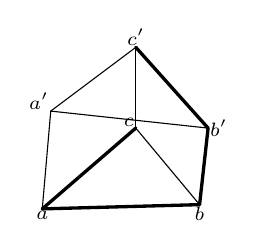
\begin{tikzpicture}[x=0.054cm,y=-0.054cm,line cap=round,line join=round,line width=.4pt]
\draw[very thick] (1,39) -- (38,38);
\draw (38,38) -- (23,20);
\draw[very thick] (23,20) -- (1,39);
\draw (3,16) -- (40,20);
\draw[very thick] (40,20) -- (23,1);
\draw (23,1) -- (3,16);
\draw (1,39) -- (3,16);
\draw[very thick] (38,38) -- (40,20);
\draw (23,20) -- (23,1);
\node[inner sep=.55pt,anchor=north,font=\scriptsize] at (1,39) {$a$};
\node[inner sep=.55pt,anchor=north,font=\scriptsize] at (38,38) {$b$};
\node[inner sep=.55pt,anchor=south east,font=\scriptsize] at (23,20) {$c$};
\node[inner sep=.55pt,anchor=south east,font=\scriptsize] at (3,16) {$a'$};
\node[inner sep=.55pt,anchor=west,font=\scriptsize] at (40,20) {$b'$};
\node[inner sep=.55pt,anchor=south,font=\scriptsize] at (23,1) {$c'$};
\end{tikzpicture}%
}}
\end{tikzcd}%
}

\unsure{prismes épinglés)|prismes épinglés}

\[
\begin{aligned}
27\cdot10\cdot8\cdot4\cdot\underline{1}&=[W]:6\\
\text{prismes}:&\quad[W]:72
\end{aligned}
\]

\diagram{%
\begin{tikzcd}[ampersand replacement=\&,column sep=0pt,row sep=0pt]
|[inner sep=0pt]| \vcenter{\hbox{%
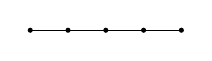
\begin{tikzpicture}[x=0.04cm,y=-0.04cm,line cap=round,line join=round,line width=.4pt]
\draw (0,0) -- (12,0) -- (24,0) -- (36,0) -- (48,0);
\fill (0,0) circle[radius=0.0325cm];
\fill (12,0) circle[radius=0.0325cm];
\fill (24,0) circle[radius=0.0325cm];
\fill (36,0) circle[radius=0.0325cm];
\fill (48,0) circle[radius=0.0325cm];
\end{tikzpicture}%
}}
\end{tikzcd}%
}

\[
\begin{aligned}
&27\cdot10\cdot8\cdot4\cdot1\\
A_5\ \text{épinglés}:&\quad[W]:6\\
A_5:&\quad[W]:12
\end{aligned}
\]

\diagram{%
\begin{tikzcd}[ampersand replacement=\&,column sep=0pt,row sep=0pt]
|[inner sep=0pt]| \vcenter{\hbox{%
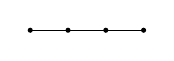
\begin{tikzpicture}[x=0.04cm,y=-0.04cm,line cap=round,line join=round,line width=.4pt]
\draw (0,0) -- (12,0) -- (24,0) -- (36,0);
\fill (0,0) circle[radius=0.0325cm];
\fill (12,0) circle[radius=0.0325cm];
\fill (24,0) circle[radius=0.0325cm];
\fill (36,0) circle[radius=0.0325cm];
\end{tikzpicture}%
}}
\end{tikzcd}%
}

\[
\begin{aligned}
A_4\ \text{épinglés}:&\quad27\cdot10\cdot8^{\inserted{4}}=[W]:\unsure{6}\\
A_4&\quad[W]:12
\end{aligned}
\]

\diagram{%
\begin{tikzcd}[ampersand replacement=\&,column sep=0pt,row sep=0pt]
|[inner sep=0pt]| \vcenter{\hbox{%
\begin{tikzpicture}[x=0.04cm,y=-0.04cm,line cap=round,line join=round,line width=.4pt]
\draw (0,0) -- (12,0) -- (24,0);
\fill (0,0) circle[radius=0.0325cm];
\fill (12,0) circle[radius=0.0325cm];
\fill (24,0) circle[radius=0.0325cm];
\end{tikzpicture}%
}}
\end{tikzcd}%
}

\[
\begin{aligned}
A_3\ \text{épinglés}:&\quad27\cdot10\cdot8=\unsure{[W]|[\mathrm{W}]}:24\\
&\text{(autres que des triangles épinglés)}\\
A_3\ \deleted{\unsure{\text{ép.}}}:&\quad[W]/48
\end{aligned}
\]

\diagram{%
\begin{tikzcd}[ampersand replacement=\&,column sep=0pt,row sep=0pt]
|[inner sep=0pt]| \vcenter{\hbox{%
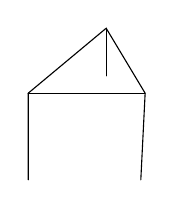
\begin{tikzpicture}[x=0.055cm,y=-0.055cm,line cap=round,line join=round,line width=.4pt]
\draw (0,35) -- (0,15) -- (18,0) -- (27,15) -- (26,35);
\draw (0,15) -- (27,15);
\draw (18,0) -- (18,11);
\end{tikzpicture}%
}}
\end{tikzcd}%
}

carroussels \inserted{simples} épinglés

\[27\cdot10\cdot8\cdot4\cdot3=[W]:2\]

carroussels \inserted{simples}\quad $[W]:12$

\diagram{%
\begin{tikzcd}[ampersand replacement=\&,column sep=0pt,row sep=0pt]
|[inner sep=0pt]| \vcenter{\hbox{%
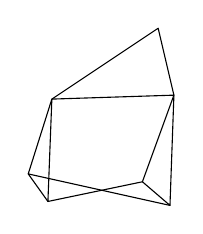
\begin{tikzpicture}[x=0.05cm,y=-0.05cm,line cap=round,line join=round,line width=.4pt]
\draw (5,37) -- (11,18) -- (38,0) -- (42,17) -- (41,45) -- (5,37);
\draw (11,18) -- (42,17) -- (34,39) -- (10,44) -- (11,18);
\draw (34,39) -- (41,45);
\draw (5,37) -- (10,44);
\end{tikzpicture}%
}}
\end{tikzcd}%
}

\unsure{$1$}

% archive sheet number: 84
